\newpage
\thispagestyle{empty}
\chapter{Quantum walks with time-dependent Hamiltonians and their application to the search problem on graphs}
The main purpose of this thesis is to study quantum walks with time dependent hamiltonians, focusing in particular on their application to the spatial search problem on graph. The general idea is trying to improve a time-independent implementation of quantum walks search using a time-dependent hamiltonian analogous to the one used in the adiabatic evolution. In order to determine whether this new approach produces successfull results we study two selected graph topology: the circular graph, for which the time-independent approach is not able to solve the search problem, and the complete graph for which the search problem is solved for both the time-independent and adiabatic evolution approaches. \\ We compare the two methods for the optimized-search, localization - which represents a search without needs to optimize the time - and a measure of robustness.

\section{Search with Time-Dependent Hamiltonian}
In Section? we discussed the use of quantum walks for the spatial search problem \cite{Childs2004} and the application to the complete graph where the search problem is solved. We then illustrated how the adiabatic theorem can be used to solve computational problems with an adiabatic evolution of a quantum system \cite{Farhi2000}. Efforts to combine the two approaches showed that the search problem can be solved only with structures stronger than the usual Grover's oracle \cite{Wong2016}, thus making an \textit{Adiabatic-Quantum-Walk-Search} impossible. However this leaves space to a merely time-dependent quantum walk search, that takes advantage of a time-dependent implementation similar to the adiabatic evolution but that is not bounded to the strict adiabatic-theorem conditions and the limitation of the standard Grover's oracle.


    \subsection{Time-Dependent Quantum Walk}
        Following from the adiabatic evolution discussed in the preliminaries, we consider a search hamiltonian that interpolates between an initial hamiltonian, i.e. the laplacian of the graph $L$, and the final oracle hamiltonian $H_w=\gamma\ket{w}\bra{w}$
          \begin{equation}
            H(s) = (1-s)L - s\gamma|w\rangle\langle w|
          \end{equation}
        where the interpolation schedule $s=s(t)$ goes from 0 to 1 as the time $t$ goes from 0 to the runtime $t_f$. \\ \\In order to find the evolved ground state of the beginning hamiltonian we need to determine the evolution operator that for a time-dependent hamiltonian is given by:
        \begin{equation}
          S(t,t_0) = \mbox{T} \mbox{exp} \frac{1}{i\hbar}\Big\{ \int_{t_0}^{t} dt' H(t')\Big\}
        \end{equation}
        where T is the time-ordering. Since we're only interested in the evolved state, having the exact evolution operator is somewhat irrelevant. Additionally for the circular graph - which represents the main topology studied in this thesis - the search hamiltonian does not show any particular properties making an analitical derivation of the operator not possible. We therefore proceed by solving the differential Schroedinger equation:
        \begin{equation}
          i\frac{d}{dt}|\psi(t)\rangle = H |\psi(t)\rangle
        \end{equation}
        Recalling that we're dealing with matrices and vectors in an N-dimensional Hilbert space, we solve N-differential equations of the form
        \begin{equation}
        \frac{d}{dt}|\psi_i(t)\rangle = \sum_jH_{ij}|\psi_i(t)\rangle
        \end{equation}
        with the boundary conditions $|\psi_i(0)\rangle = |\psi_i\rangle$.\\
        From a numerical point of view this approach is also much simpler than other direct methods of evaluating the evolution operator, such as the Dyson Series or Magnus Expansion.




    \subsection{Interpolating Schedule s(t)}
        As pointed by Wong the interpolating schedule s(t) plays a crucial role in the evolution of the system and in the overall scaling of the algorithm.
        The original adiabatic evolution by Farhi and Gutmann. \cite{Farhi2000} uses a linear interpolating schedule defined as $s(t) = \frac{t}{t_f}$. Ronald and Cerf show that in order to obtain a quadratic speedup for the complete graph a non linear schedule is essential \cite{Roland2002}\cite{Morley2018}.

        Thus, from a linear interpolating schedule we begin considering, somewhat naively, quadratic and cubic schedules:
        \begin{equation}
          s(t) = \sqrt{\frac{t}{t_f}} \hspace{30pt} s(t) = \sqrt[3]{\frac{t}{t_f}}
        \end{equation}
        We then consider the interpolating schedule analitically derived by Ronald and Cerf for the unstructured search (complete graph) given by :
        \begin{equation}
            t = \frac{1}{2\epsilon}\frac{N}{\sqrt{N-1}}\Big[\mbox{arctan}\big(\sqrt{N-1}(2s-1)\big) + \mbox{arctan}\sqrt{N-1}\Big]
        \end{equation}
        By inverting the function, $s(t)$ is obtained as plotted in \cref{cerf}(a) \\
        The shape of this interpolating schedule comes from the gap $g(s)$ between the lowest two eigenvalues, changing faster when the gap is large, while it evolves slower when the gap is small. We therefore take these key aspects of $s(t)$ - derived for the unstructured search - an consider a similar interpolating schedule defined as follow
        \begin{equation}
            s(t) = \frac{1}{2}(2(x-1)^{3}+1)
        \end{equation}
        \begin{figure}[ht]
          \centering
          \begin{tabular}{cc}
            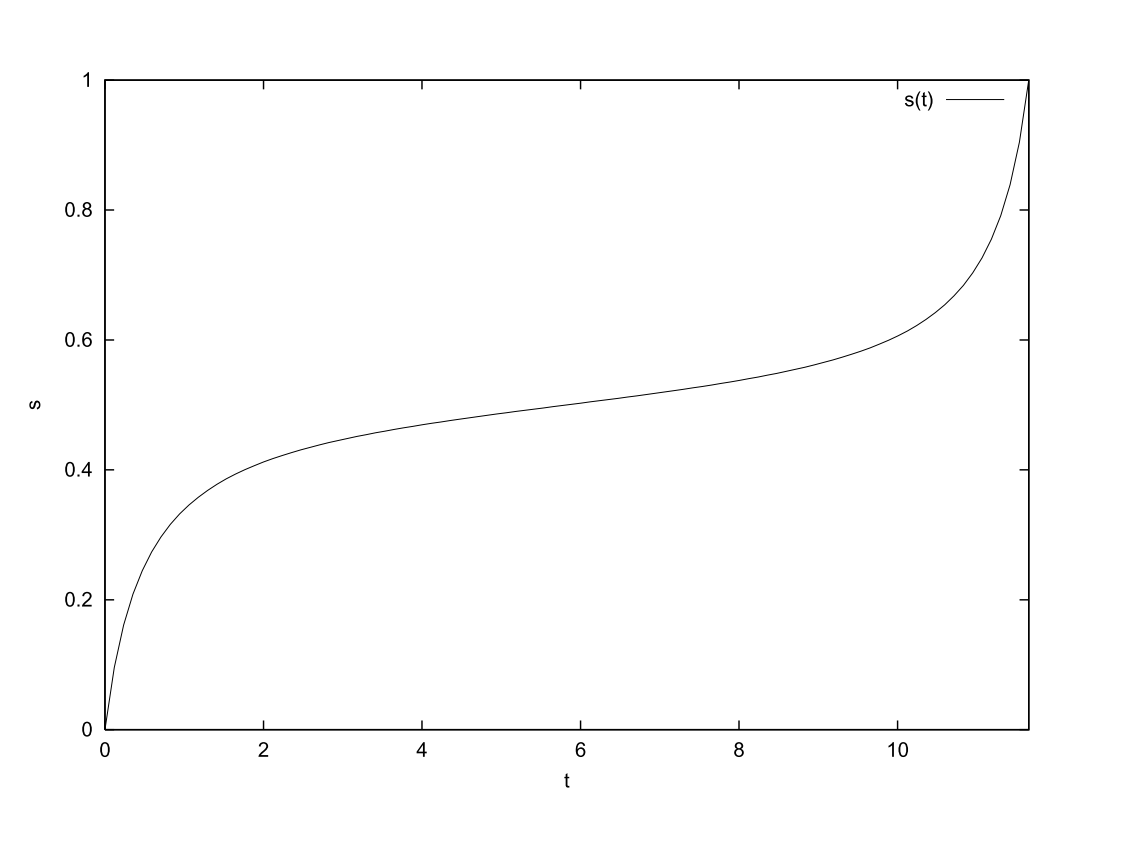
\includegraphics[width=75mm]{./figures/interpolating_schedules/cerf} &   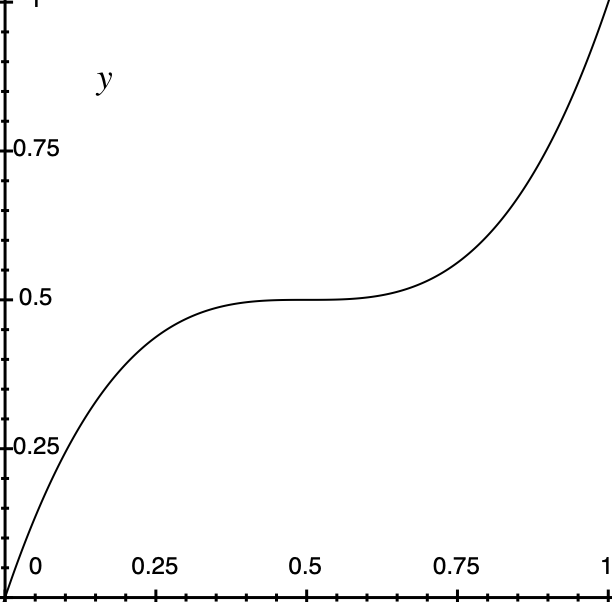
\includegraphics[width=45mm]{./figures/interpolating_schedules/our_cerf} \\
          (a) Original Ronald-Cerf & (b) Ronald-Cerf like\\[6pt]
          \end{tabular}
          \caption[Ronald and Cerf's interpolating schedules for the unstructured search and our non-linear schedule]{\textbf{Ronald and Cerf's interpolating schedule (a) and our Ronald-Cerf like schedule (b).} These figures show the difference between the original interpolating schedule derived by Ronald and Cerf for the unstructured search (left) and our Ronald-Cerf like schedule(right). Although quite different we study the effects of this particular non-linear interpolating schedule and compare it with the linear one used by Farhi and Gutmann \cite{Farhi2000}.}
          \label{cerf}
        \end{figure}

        \subsection{Multiple Runs for One Search}
        To give a complete picture of the usefulness of the time-depedent approach, we consider the possibility of repeating the search multiple times. If the probability at which the solution is found is $p=1$ the search is perfect and the problem is solved. However, if the proabability is less than one, i.e. imperfect search, the problem can be solved by searching multiple times . Since the results of the search are checked independently, a single successfull search is sufficient, and this kind of routine is efficient as long as the probability $\big|\langle\psi(t_f)| w\rangle\big|^2$ is greater than $1/poly(N)$ (where N is the dimension of the graph) \cite{Morley2018}.

        Repeating the search multiple times does however come at a cost. It is indeed necessary to take into account for a non-zero \textit{initialization} time $t_{init}$ to prepare the system in the correct state as well a physical time for the measurement. Therefore, computing multiple searches with small $t_f$ becomes less efficient than less searches with larger $t_f$, where the quantity $t_{init}$ makes a lesser contribution to the overall $t_f$. Clearly this consideration is particularly relevant for increasing graph size.

\section{Selected Topology: Circular and Complete Graph}
    Throughout our analysis we will focus the attention on two selected graph topology, the ring graph (R) and the complete graph (C). \\

    As previously discussed in Section? the \textbf{complete graph} represents the best case scenario since it has been shown to solve the search problem both for the standard time-independent quantum walk approach \cite{Childs2004} and the local adiabatic evolution \cite{Roland2002}, with a quadratic speed up. An adiabatic implementation of the quantum walk search does not work with the usual Grover's oracle requiring a more elaborate structure \cite{Wong2016}, however as we shall later see a merely time-dependent approach might give promising results in terms of robustness.  \\

    The \textbf{circular graph} on the other hand is not able to solve the search problem with the time-independent approach, and can give some interesting insights with the application of the time-dependent quantum walk search.  \\

    The choice of graph topology is therefore based on the idea of giving results at either side of the spectrum of 2-dimensional graphs, trying to improve a non-working approach on one side, and get some interesting insights on an already perfect-search approach on the other.

\section{Characterization of the results: Search, Localization and Robustness}
    Firstly it's necessary to define what type of results we're looking for. We begin by shwoing the difference between \textbf{search} and \textbf{localization}. Then we introduce a (not-so-rigorous) measure for the \textbf{robustness} of the search algorithm.

    \subsection{Search vs Localization}
      Before looking at the results it's necessary to characterize two particular classes of results, the \textbf{search} and the \textbf{localization}, that help us decide whether the time-dependent approach does bring any advantages.
      \begin{itemize}
          \item the (optimized) \textbf{search} describes the usual search, namely the finding of the solution with high probability (possibly unitary) for the smallest time as possible. As previously mentioned we also take into account the possibility of repeating the search multiple times.
          \item the \textbf{localization} describes the finding of the solution with high probablity without the need to optimize the time. This description becomes necessary if we take into account the adiabatic nature of the time-dependent approach, that guarantees unitary probability for large enough $t_f$.
      \end{itemize}

    \subsection{Robustness}
        We've seen that the probability of a search problem depends on the time $t_f$ at which the quantum state is measured and the parameter $\gamma$. The optimal probability, i.e. highest possible, clearly is given by the optimal combination $t_f-\gamma$, and since the time $t_f$ should not be bound to errors give it's the time at which the state is measured, fluctuations in the probability are necessarily caused by fluctuations in the $\gamma$ parameter. \\
        Following from \cite{SH.HungS.Hietala2019} we define the \textbf{robustness} as quantitative measure representing the variation on the probability due to some perturbation/noise on $\gamma$.
        We begin by finding the optimal probability $P$, evaluated with the single or multiple run for one search approach. For the corresponding $(t_f,\gamma)$ combination we evaluate the robustness as follows:
        \begin{equation}
            R ^\pm = P(t_f, \gamma) - P(t_f, \gamma \pm \delta)
        \end{equation}
        where $\delta$ is some positive perturbation of the $\gamma$ parameter. As we shall later see this quantity is given in terms of some percentage of $\gamma$. To find a unique value for the robustness an average of $R^\pm$ is done:
        \begin{equation}
            R = \frac{R^++ R^-}{2}
        \end{equation}
        The quantity R should be positive, since the $(t_f,\gamma)$ combination should produce the highest probability possible. We also that the perturbation on the parameter has equal probability of being positive or negative, thus the average ponderates between these two possibilities. \\ \\It is necessary however to remember that the value $R$ does not have any absolute physical significance, but fits well for our specific scenario where the interest is focused on the comparison between two specific approaches. Therefore this quantity will be solely used to characterize a particular approach as \textbf{more} or \textbf{less robust}.

\section{Results for the Circular Graph}
We now address the results for the circular graph. We begin by computing benchmarks for the time-independent hamiltonian approach; this should give us a good starting point for the comparison. Then we consider the time-dependent hamiltonian and evaluate the necessary data. We compare the two approaches, beginning from the Localization, followed by the Search which requires the introduction of a new quantity that takes into account the possibility of doing multiple runs for one search. Lastly we study the robustness of the time-dependent approach and determine whether the newly introduced hamiltonian makes the search more robust than the time-independent search.

    \subsection{Time-Independent Benchmarks}
        The first step of the analysis is to compute time-independent benchmarks. We computed the probability over a time-beta grid, with $T\in[0,N]$ and $\gamma\in[0,2.5]$, where N is the dimension of the graph considered. An initial run of the probability distribution showed that the probability does not increase with time, thus the need to evaluate for $t_f$ greater than $T=N$ proved to be unnecessary. In addition Grover algorithm for the unstructured search (and the complete graph) scales $\sqrt{N}$ and the Farhi and Gutmann's adiabatic evolution scales like $N$, thus focusing on $T \leq N$ made much more sense. \textbf{Figure of probability distribution for sampled $\gamma$} \\
        Throughout the analysis we will consider graphs up to N = 71, with only odd dimensions which makes a easier oracle placement. Additional considerations and reasoning for the time-gamma grid can be found in Appendix A. \\


        To display the results in an intuitive way we used a heatmap plot, which gives a good idea on the probability distribution for varying combinations of $(T,\gamma)$:

          \begin{figure}[ht]
            \centering
            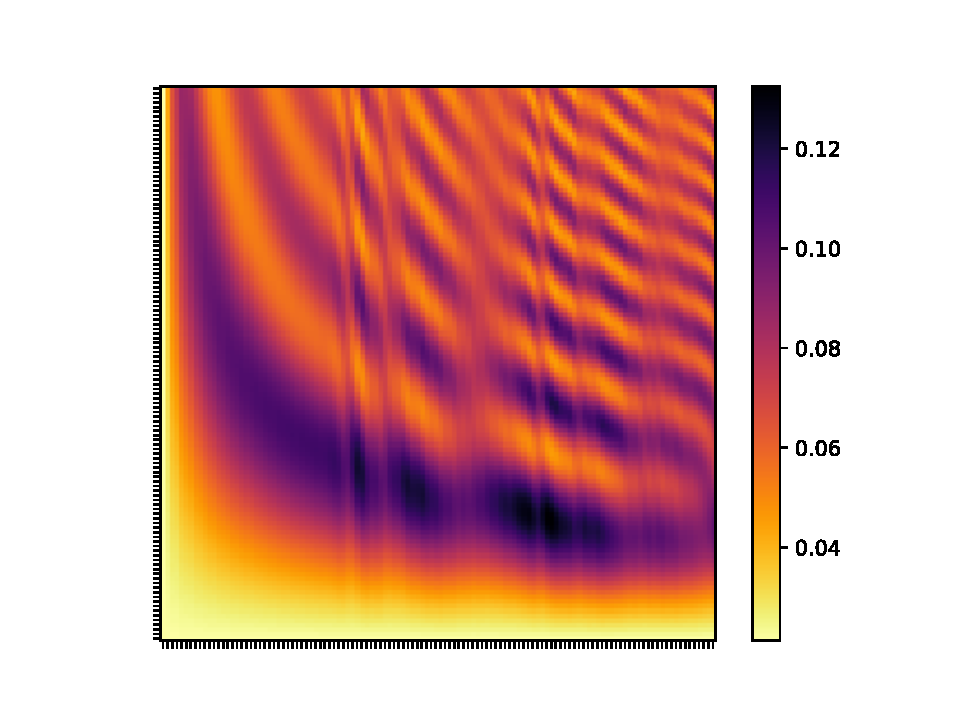
\includegraphics[width=9cm]{./figures/time_independent_benchmark_47}%
            \caption[Probability heatmap plot for the time-independent hamiltonian, N=47]{\textbf{Probability heatmap plot for the time-independent hamiltonian.} The figure shows the probability distribution for a circular graph of N=47 evaluated using the time-independent hamiltonian, providing thus the necessary benchmark. Note that dark color do not represent probabilities close to one, but only higher probability regions.}
          \end{figure}

        \subsubsection*{Comments on the probability distribution}
        From the heatmap plot we see that the probability distribution does not increase smoothly with increasing time, but shows peaks (dark regions) and valleys (lighter regions). Additionally dark regions are scattered throughout the grid and not necessarily for large $t_f$. We will later see that this is somewhat a weakness of the time-independent approach, since a small variation of the parameter $\beta$, which reperesents as previosly mentioned the deepness of the well or an energy parameter, leads to possibly great variation of the probability.

    \subsection{Time-Dependent Results}
        Similarly we computed the grid probability using the time-dependent hamiltonian previously introduced. To easily comparing the two methods we opted to consider the same time $T=N$, and from an initial run we discovered that the $\gamma$ parameter affected similarly the probability \textbf{(A plot is needed to support this statement)}, namely the probability tended to be higher for smaller values of $\gamma$, thus we used approximately the same range. \\

        The grid-probability is evaluated for all the interpolating schedules $s(t)$ previsouly discussed, and an intuitive heatmap plot is outputted.
        \begin{figure}[ht]
        \centering
        \begin{tabular}{cc}
          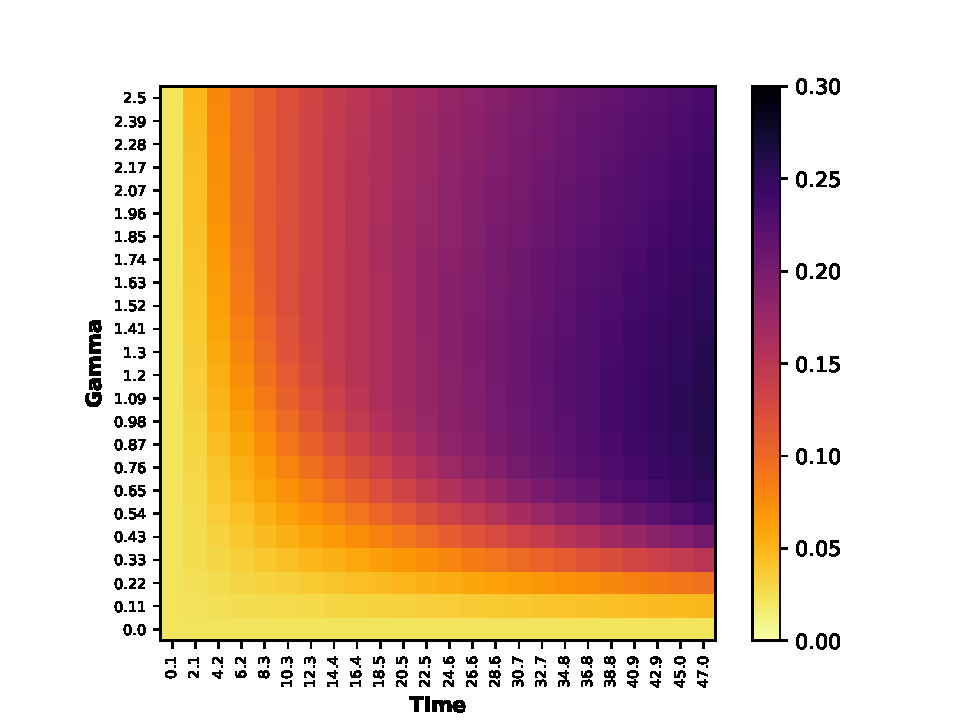
\includegraphics[width=75mm]{./figures/time_dependent_heatmap/47_heatmap_time_dependent_lin.pdf} &   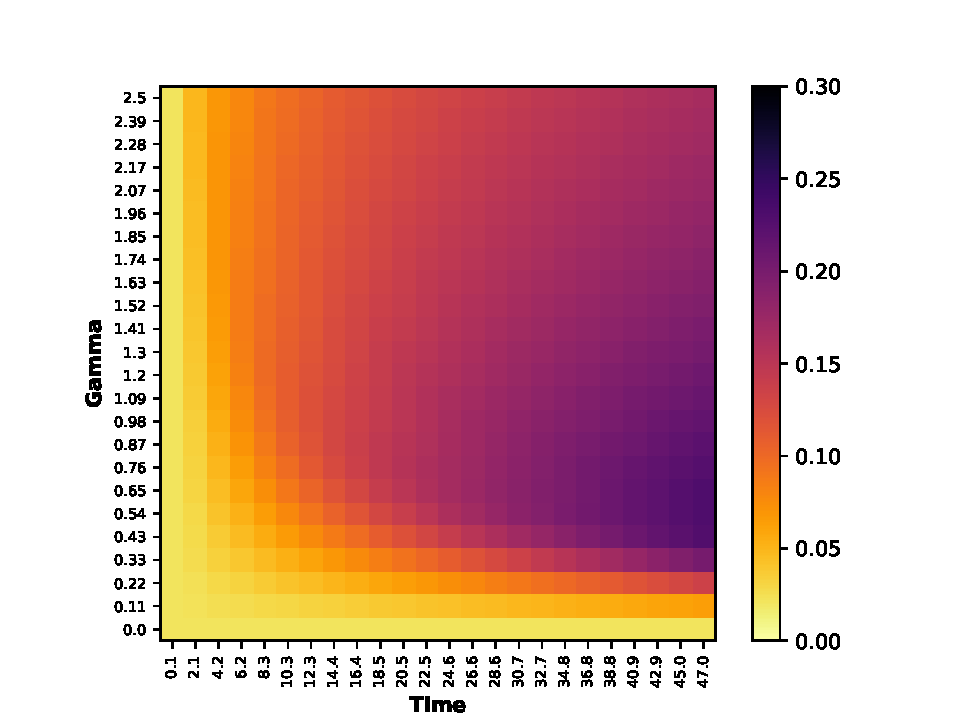
\includegraphics[width=75mm]{./figures/time_dependent_heatmap/47_heatmap_time_dependent_sqrt.pdf} \\
        (a) lin & (b) sqrt\\[6pt]
        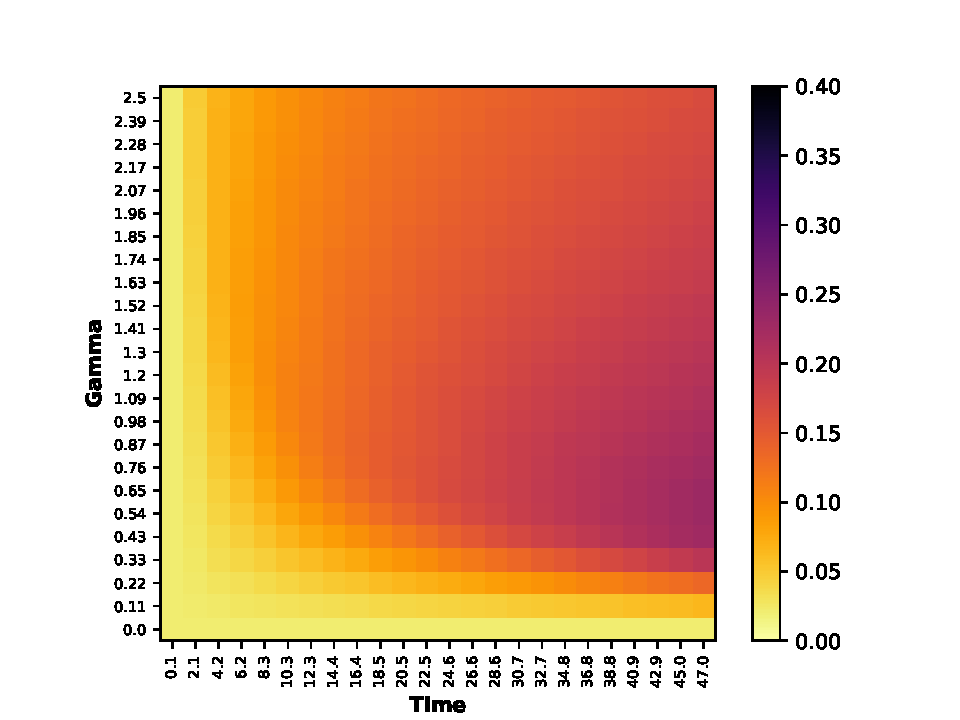
\includegraphics[width=75mm]{./figures/time_dependent_heatmap/47_heatmap_time_dependent_cbrt.pdf} &   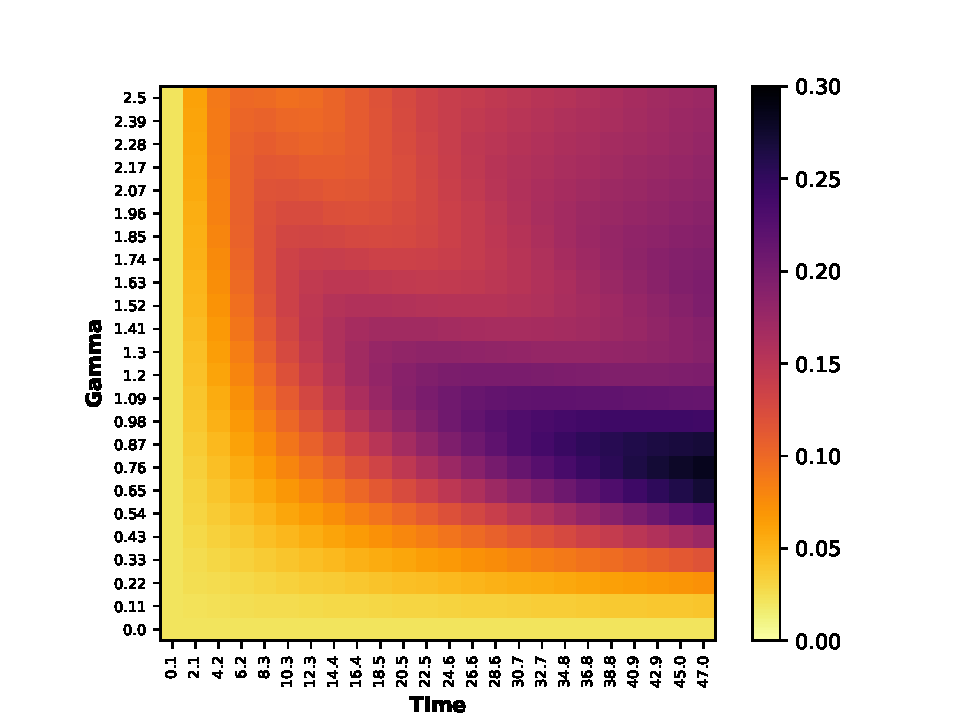
\includegraphics[width=75mm]{./figures/time_dependent_heatmap/47_heatmap_time_dependent_cerf.pdf} \\
        (c) cbrt & (d) cerf\\[6pt]
        \end{tabular}
        \caption[Probability heatmap plot for the time-dependent hamiltonian, for different shapes of s(t)]{\textbf{Probability heatmap plot for the time-dependent hamiltonian, for different shapes of s(t).} The figure shows the probability distribution for a circular graph of N=47 evaluated using the time-dependent hamiltonian using the following step functions (a) linear, (b) $\sqrt{t/T}$, (c) $\sqrt[3]{t/T}$ and (d) Ronald-Cerf(3). Note that the color gradient is normalized to p=0.3 to accentuate the difference in probability between different regions. }
        \label{time_dependent_heatmap}
        \end{figure}\\
        \subsubsection*{Comments on the probability distribution}
        Compared to the time-independent hamiltonain approach we can clearly see that the probability distribution is smoother (has no valley and peaks) both for constant $\gamma$ (any orizontal section) and constant $t_f$ (any vertical section). If we look at the different interpolating schedules it's immediately evident that the cbrt and sqrt schedules perform poorly compared to the linear one. On the other hand the Ronald-Cerf schedule performs in a similar way in terms of the highest probability found, but has a significantly different probability distributio, that might affect its robustness.
        \clearpage
    \subsection{Comparison: Localization}
        We now compare the localization properties of the two algorithm. As we mentioned in the comments to the probability distributions of the time-independent and time-dependent approaches we discovered the following:
        \begin{itemize}
            \item \textbf{Time-Independent QW}: the time-independent based search is not able to solve the search problem with a single iterations, thus making it necessary to run multiple searches. This implies that the approach does not show any localization properties, in fact the probability does not increase with time as in the time-dependent approach.
            \item \textbf{Time-Dependent QW}: the time-dependent based search on the other hand because of the adiabatic theorem does solve the search problem with a single iterations, although that happens for fairly large $t_f$.
        \end{itemize}
        Although the time-dependent approach is able to get to unitary probability in a fairly large $t_f$, it is able to produce large enough probabilities in much less time, as we can see from this plot. This is a consequence of the fact that the probability does not grow linearly with time, thus needing larger $t_f$ closer it gets to $P=1$. \textbf{A plot is needed}


    \subsection{Comparison: Search}
        In order to compare the two approaches for the search it is clear that we cannot simply consider the time at which the solution is found with unitary probability, since that particular $t_f$ is not optimized for the time-dependent approach and does not exist for the time-independent one. Therefore, as previously mentioned we consider the possibility of doing multiple runs for one search. For this reason we introduce the following quantity
        \begin{equation}
          \min\Big(\frac{t_f}{p}\Big)
        \end{equation}
        where $1/p$ is the number of iterations necessary to get to unitary probability (statistically), and combining it with $t_f$ gives the total time necessary. Optimizing over the combination of $t_f$ and $p$ gives the smallest time necessary to get to unitary probability using the multiple search approach. Additionally, the number of iterations $\mbox{iters}=1/P$ might give some useful insights on the performance of the approach, in particular if you take into account the initialization time $t_{init}$\\ \\  However, this particualar approach poses a few problems. Infact if we look at how the quantity $t_f/p$ varies for varying $t_f$, we discover that the minimum of such quantity will always be for the smallest $t_f$ available, regardless of the type of hamiltonian and step function $s(t)$. The following plot does indeed show, for a few sampled $\gamma$, the shape of $t_f/p$. In addition, in Section ? we mentioned that when dealing with multiple runs for one search we need to take into account an initialization time $t_{init}$. It is thus necessary to consider a lower bound on $t_f$.
        \begin{figure}[ht]
        \centering
        \begin{tabular}{cc}
          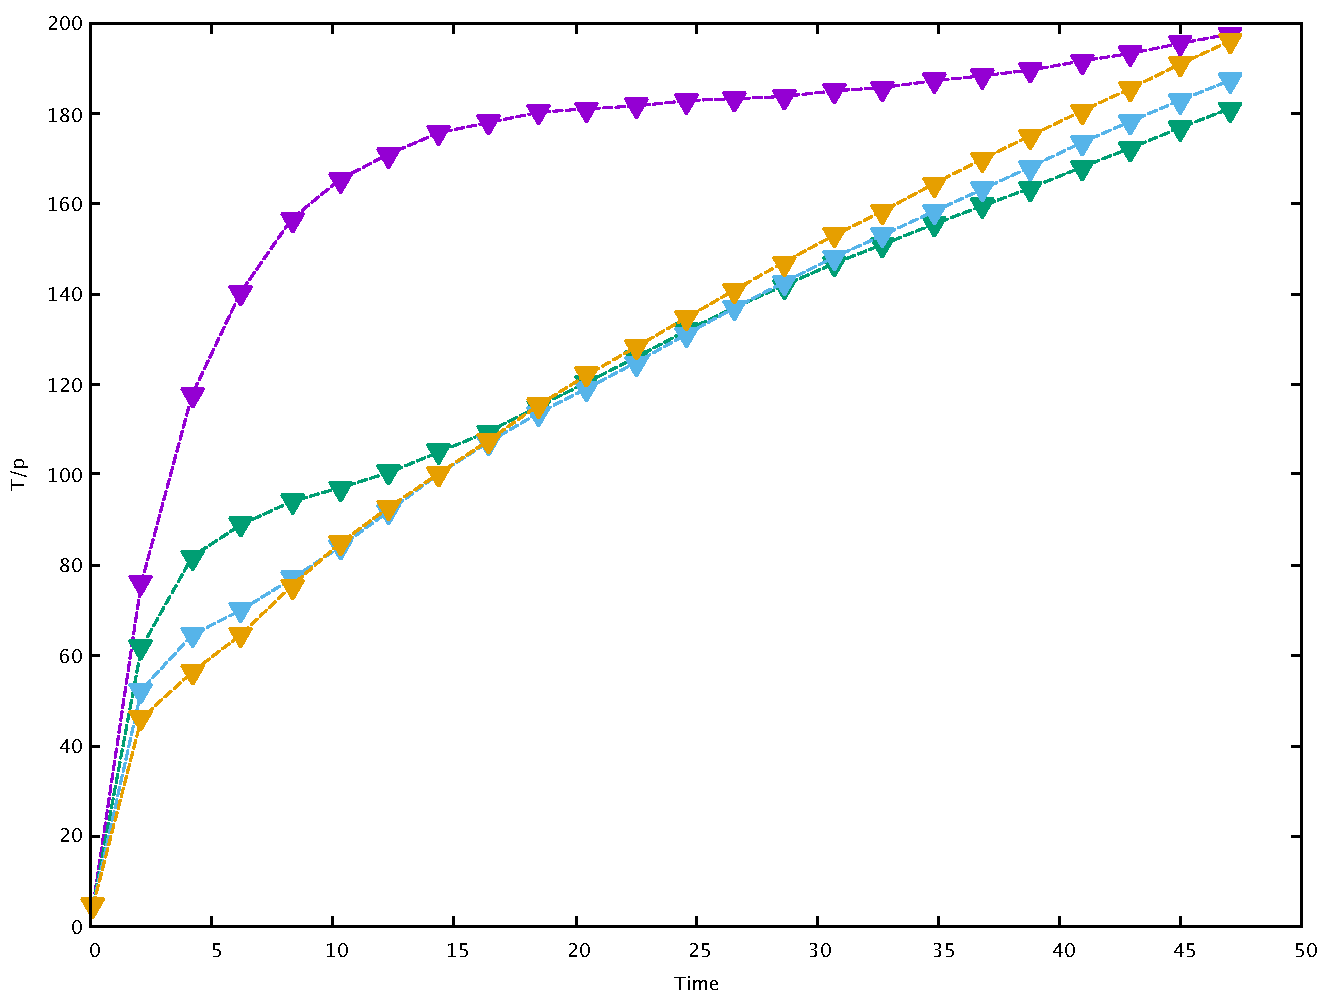
\includegraphics[width=75mm]{./figures/sampled_t_over_p/T_p_lin.pdf} &   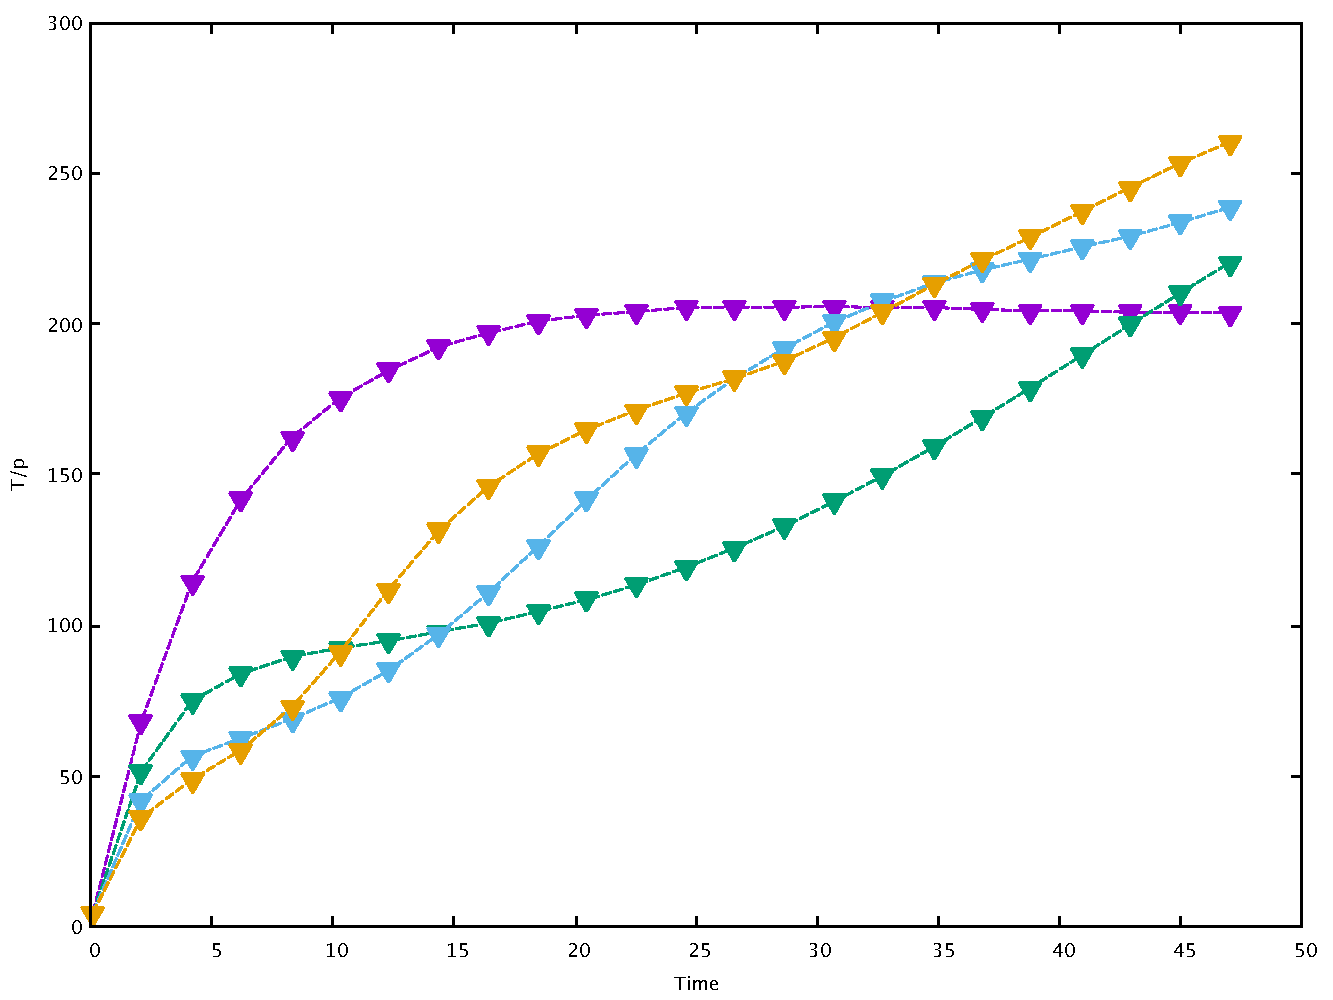
\includegraphics[width=75mm]{./figures/sampled_t_over_p/T_p_cerf.pdf} \\
        (a) lin & (b) Ronald-Cerf\\[6pt]
        \end{tabular}
        \caption[$t_f/p$ distribution for sampled $\gamma$ showing that the minimum will always be for the smallest $t$ ]{\textbf{Distribution of the quantity T/p for sampled $\gamma$ showing that tthe min(T/p) will always be the smallest for the smallest $t$.}he figure shows the distribution of the quantity $t_f/p$ for some sampled values of the parameter $\gamma$, using the linear and Ronald-Cerf interpolating schedules. It is clear that the quantity $\min(t_f/p)$ will always be for the smallest $t_f$ available, regardless of the interpolating schedule, requiring therfore a constrain on the time.}
        \end{figure}

        \bpar{\bm{$\min(t_f/p)$}  and run iterations for increasing lower bound \bm{$t_f$}}
         We will begin by studying how the quantity $\min(t_f/p)$ and $iters$ varies with increasing lower bound $t_f^*$.
         In the following plot we show the shape of $t_f/p$ with the time-independent approach and the time-dependent one; for the time being and for sake of semplicity, we consider only the step function Ronald-Cerf(3).

         %TAU LOWER BOUND TIME
         %%
%INTERPOLATING SCHEDULES: ORIGINAL ROLAND-CERF AND OUR S_RC
%%
\begin{figure}[ht]
  \centering
  \begin{tikzpicture}
    \begin{axis}[name=plot,
    xmin=0, xmax=60,
    ymin=0, ymax=600,
    width = 120mm,
    xlabel = Dimension $N$,
    ylabel = $\bm{\tau}$ ]
    \addplot[color=arancio,mark=*,mark size=2.5pt, x=a ,y=b] table{./Data/51_tau_lbt_static.txt};\addlegendentry{time-independent}
    \addplot[color=rossoscuro,mark=*,mark size=2.5pt, x=a,y=b] table{./Data/51_tau_lbt.txt};\addlegendentry{$s_L(t)$}

    \end{axis}
  \end{tikzpicture}
  \caption[$\tau$ distribution for increasing lower bound time.]{\textbf{\bm{$\tau$} distribution for increasing lower bound time. }The figure shows the $\tau$ distribution for increasing values of lower bound time, using the time-independent hamiltonian (orange) and time-dependent hamiltonain (red) and evaluated for a Cy(51). We see that for times smaller than a characteristic time $T^*$ the time-independent approach performs slightly better, while for large time the time-dependent one performs significantly better.}
  \label{fig:tau_increasing_time}
\end{figure}


        As we can see from the plot the distribution can be diveded into to section marked by a particular $T^*$ (for the time being the value of such time is not of our interest):
        \begin{itemize}
            \item for $t_f<T^*$ the time-independent approach performes slightly better than the time-dependent one.
            \item for $t_f>T^*$ however the time-dependent approach performs significantly better, in particular with increasing time $t_f$
        \end{itemize}
        The behaviour for large T is to be expected, considering that the time-dependent approach shows localization properties and the probability increases with increasing time as we shoed in Figure?, in contrast with the time-independent approach that does not show localization propeties.\\ What this show is that the choice of $t_f$ has great effects on the outcome of our time-dependent approach, making it a successfull or unsuccesfull alternative.
        In terms of iterations the trend is similar to the quantity \quantity, as the following plot shows.

        %PLOT ITERATIONS FOR LOWER BOUND TIME increasing
        %%
%TIME INDEPENDENT: PROBABILITY FOR SAMPLED GAMMA
%%

%ITERS I DISTRIBUTION FOR INCREASING LOWER BOUND TIME

\begin{figure}[ht]
  \centering
  \begin{tikzpicture}
    \begin{semilogyaxis}[name=plot
    xmin=0, xmax=60,
    ymin=0, ymax=55,
    width = 120mm,
    xlabel = Dimension $N$,
    ylabel = $\bm{I}$ ]
    \addplot[color=verdescuro,mark=*,mark size=2.5pt, x=a ,y=b] table{./Data/51_iters_lbt_static.txt};\addlegendentry{time-independent}
    \addplot[color=bluscuro,mark=*,mark size=2.5pt, x=a,y=b] table{./Data/51_iters_lbt.txt};\addlegendentry{$s_L(t)$}

    \end{semilogyaxis}
  \end{tikzpicture}
  \caption[$I$ distribution for increasing lower bound time.]{\textbf{$\bm{I}$ distribution for increasing lower bound time. }The figure shows the distribution of $I$ for increasing values of lower bound time, using the time-independent hamiltonian (green) and time-dependent hamiltonain (blue) and evaluated for a Cy(51). This distribution reflects the probability distribution of the two approaches: for the time-independent hamiltonian the probability does not increase with time, resulting in a (almost) constant $I$, while the time-dependent hamiltonian showing localization properties requires less iterations to get to unitary probability.}
  \label{fig:iters_increasing_time}
\end{figure}


        The iterations distribution reflects the overall probability distribution of the time-dependent and time-independent hamiltonian approaches. For small lower bound time the two approaches show a similar performance: the probability is very small, thus requiring a large number of iterations to get to unitary probability. As $t_f$ increases we see two very different trends:
        \begin{itemize}
            \item The time independent approach requires an almost constant number of iterations (the numerical values is somewhat irrelevant since this distribution reflects only the Cy(53) and Cy(55)). This reflects the non-localization properties of this particular approach, for which the probability does not increase with time
            \item On the other hand the time-dependent approach, showing localization properties, requires less iterations to solve the search with unitary probability.
        \end{itemize}
        Taking into account that we're performing a multiple run search and the initialization time $t_{init}$ previously discussed, it is clear that the time-depedent approch performs better than the time-independent counter part in most of the scenario.
        \clearpage
        \bpar{\bm{$\min(t_f/p)$} and run iterations with constrained lower bound time}
        In order to show that the lower bound time does indeed have such great impact on the performance of the time-dependen approach relative to the time-independent one we now study the distribution of the quantity $\min(t_f/P)$ with a constrain on the lower bound time. \\ The choice of constrain is arbitrary and somewhat biased since the larger the constrain the better the performance of the time-dependent approach, as we've just shown in \cref{fig:delta_increasing_time}. Therefore, to make the choice fair, we consider the lower bound time to be $t_f^* = 2\sqrt{N}$ which is (roughly) the time scaling of the standard Grover's Search, the QW Search on the complete graph and so on. In the best case scenario we discover that the number of iterations necessary to get to unitary probability remain constant regardless of the dimension of the graph, making this approach scale as the ones just mentioned; in the most probable scenario we discover that the number of iterations increase with the graph size, thus adding a scaling factor that depends on some power of N. \\ \\ The following plot shows the distribution of the quantity $\min(t_f/P)$ for circular graphs Cy(N) with N up to 71. The quantity is computed using the time-dependent hamiltonian with linear step function and the time-independent one, with constrained time $t_f=2 \sqrt{N}$.

        %TAU STATIC AND CERF WITH CONTRAINED TIME
        %%
%TIME INDEPENDENT: HEATMAP PLOT
%%


\begin{figure}[!htb]
  \centering
  \begin{tikzpicture}
    \begin{axis}[name=plot,
    zmin=0,zmax=1,
    view={0}{90},
    colormap={inferno}{rgb255=(248,251,155) rgb255=(251,179,21) rgb255=(236,103,38) rgb255=(187,54,84) rgb255=(119,29,109) rgb255=(49,9,92) rgb255=(1,1,8)},
    point meta min=0,
    point meta max=0.25,
    colorbar,
    colorbar style = {ylabel=Probability, ytick={0.02, 0.04, 0.06, 0.08, 0.1}},
    width = 80mm,
    height= 80mm,
    xlabel = $\bm{T}$,
    ylabel = $\bm{\gamma}$
    ]
    \addplot3 [surf] table[x=a,y=b,z=c]{./Data/fig3/51_heatmap_static.txt};

    \end{axis}
  \end{tikzpicture}
  \caption{\textbf{Probability distribution for the time-independent Hamiltonian}. The figure shows the probability distribution for the cycle graph $Cy(51)$ evaluated using the time-independent Hamiltonian, providing the necessary benchmarks. Note that dark color regions do not represent probabilities close to one.}
  \label{fig:heatmap_time_independent}
\end{figure}


        \bpar{\bm{$\min(t_f/p)$} and run iterations for different shapes of s(t)}
        We now investigate the effects of the different step functions discussed in section? in the probability distribution and in particular on the quantity $\min(t_f/P)$. As we did for the general time-dependent and time-independent comparison we constrain the lower bound time to be larger than $2\sqrt{N}$.
        The following plot shows the distribution of the quantity $\min(t_f/P)$ for circular graphs Cy(N) with N up to 71, using the time-dependent hamiltonian with linear, sqrt, cbrt and Ronald-Cerf(3) interpolating schedules $s(t)$:

        %TAU CONSTRAINED TIME - DIFFERENT INTERPOLATING SCHEDULES
\begin{figure}[ht]
  \centering
  \begin{tikzpicture}
    \begin{axis}[name=plot
    xmin=0, xmax=80,
    ymin=0, ymax=360,
    width = 120mm,
    height = 95mm,
    xlabel = Dimension $N$,
    ylabel = $\bm{\tau}$,
    legend style={at={(0,1)},
    anchor=north west}]
    \addplot[color=verdescuro,mark=*,mark size=2.5pt, x=a, y=b] table{./Data/tau_linear.txt};\addlegendentry{$s_{L}(t)$}
    \addplot[color=bluscuro,mark=*,mark size=2.5pt, x=a, y=b] table{./Data/tau_sqrt.txt};\addlegendentry{$s_{S}(t)$}
    \addplot[color=rossoscuro,mark=*,mark size=2.5pt, x=a, y=b] table{./Data/tau_cbrt.txt};\addlegendentry{$s_{C}(t)$}
    \addplot[color=arancio,mark=*,mark size=2.5pt, x=a, y=b] table{./Data/tau_cerf.txt};\addlegendentry{$s_{RC}(t)$}

    \end{axis}
  \end{tikzpicture}
  \caption[$\min(t_f/P)$ distribution for Cy(N) up to N=71 with constrained time at $\sqrt(N)$ and different interpolating schedules.]{\textbf{\bm{$\min(t_f/P)$} distribution for Cy(N) up to N=71 with constrained time at $\bm{2\sqrt{N}}$ and different interpolating schedules.} The figure shows the distribution of the quantity min(T/p) with constrained lower bound time at $t_f= 2\sqrt{N}$, using the time-independent hamiltonian and time-dependent hamiltonain with different interpolating schedules. The abrupt changes are due to the resolution of the grid-probability evaluation (further discussions can be found in Appendix A)}
  \label{fig:delta_complete_sqrt}
\end{figure}


        \noindent
        We can see from the plot that, as we might have expected, the Ronald-Cerf interpolating schedule performes better than the linear and sqrt schedules, in particular when we consider larger graph. For small enough N the time-independent approach performs slightly better, while for large N the time-depenedent approach is superior. Please note that the abrupt changes in the plot are due to the resolution of the grid-probability evaluation, discussed in Appendix A. \textit{nota: Additional computations will be run to try to fix this issue}.


    \subsection{Comparison: Robustness}
    We now address the robustness of the time-dependent and time-independent search. As we mentioned in Section? we're only interested in the comparison of the two approaches, and not an absolute measure of their robustness. Therefore we will use this measure solely as a comparison value. \\
    We proceed by considering small variations on the parameter $\gamma$ in the order of 1\% and 5\% (this numbers still need to be discussed). We begin by finding the quantity $\min(t_f/P)$ with time constrains ($t_f = 2\sqrt{N}$). For the corresponding $(t_f,\gamma)$ combination we evaluate the robustness R as defined in Section?
    For the time-dependent search with only consider the linear step function an the Ronal-Cerf(3). As we showed in the previous section the Ronald-Cerf Hamiltonian performs better than the linear conterpart, while from a qualitative point of view the linear hamiltonian has a smoother probability distribution (see \cref{time_dependent_heatmap}(a)-(d)). The following plots show the semi-quantitative robustness for the $\gamma$ variations in the order of 1\% - 5\% for the time-independent search and the time-dependent one with linear and Ronald-Cerf step functions s(t). \textbf{Computations are still needed}

    %ROBUSTNESS PLOT
    %%
%PROBABILITY DISTRIBUTION FOR SAMPLED N, UP TO P=1
%%

\begin{figure}[ht]
\centering
  \begin{tikzpicture}
    \begin{axis}[name=plot
    xmin=0, xmax=441,
    ymin=0, ymax=1,
    width = 120mm,
    height=95mm,
    xlabel = $\bm{T}$,
    ylabel = $\bm{p}$,
    legend style={at={(0.95,0.05)},
    anchor=south east}]
    \addplot[color=verdescuro,no marks, thick, x=a, y=b] table{./Data/fig6/fig6_21_lin.txt};\addlegendentry{$N=21$, $\gamma=1.5$, $s_L(t)$}
    \addplot[color=verdescuro,dashed, no marks, thick, x=a, y=b] table{./Data/fig6/fig6_21_cerf.txt};\addlegendentry{$N=21$, $\gamma=1.05$, $s_{RC}(t)$}

    \end{axis}
  \end{tikzpicture}
  \caption{\textbf{Probability distibution for a $\bm{Cy(21)}$ with sampled $\bm{\gamma}$}: The figure shows the probability distribution for the cycle graph $Cy(21)$, evaluated with the time-dependent hamiltonian using the interpolating schedules (solid) linear $s_L$ and (dashed) Roland-Cerf $S_{RC}$. We can see that the probability increases with time, as expected. }
  \label{fig:probability_sampled_gamma}
\end{figure}



\section{Results for the Complete Graph}
    \subsection{Search results from Wong(2016)}
    \subsection{Localization results}
